% To je predloga za poročila o domačih nalogah pri predmetih, katerih
% nosilec je Blaž Zupan. Seveda lahko tudi dodaš kakšen nov, zanimiv
% in uporaben element, ki ga v tej predlogi (še) ni. Več o LaTeX-u izveš na
% spletu, na primer na http://tobi.oetiker.ch/lshort/lshort.pdf.
%

\documentclass[a4paper,11pt]{article}
\usepackage{a4wide}
\usepackage{fullpage}
\usepackage[utf8x]{inputenc}
\usepackage[slovene]{babel}
\selectlanguage{slovene}
\usepackage[toc,page]{appendix}
\usepackage[pdftex]{graphicx} % za slike
\usepackage{setspace}
\usepackage{color}
\definecolor{light-gray}{gray}{0.95}
\usepackage{listings} % za vključevanje kode
\usepackage{hyperref}
\usepackage{titlesec}
\usepackage{enumitem}

\renewcommand{\baselinestretch}{1.2} % za boljšo berljivost večji razmak
\renewcommand{\appendixpagename}{\normalfont\Large\bfseries{Priloge}}

% Naloga
\author{Sebastian Mežnar, IŠRM}

\title{
Uporaba umetne inteligence za zmago igre 2048\\
\large Seminarska naloga pri predmetu Osnove umetne inteligence\
\large Šolsko leto 2018/19
}

\date{\today}

\begin{document}

\maketitle

 \section{Povzetek} 
2048 je preprosta računalniška igra v kateri združuješ skupaj ploščice tako, da iz dveh z istim številom dobiš novo, na kateri je seštevek obeh. Cilj te igre je narediti ploščico z številom 2048. V nalogi sem to igro poiskušal zmagati s pomočjo hevrističnega preiskovalnega algoritma. Del programske kode z igro sem našel na spletu, saj je ta igra odprtokodna, algoritem za iskanje najboljše poteze sem pa implementiral sam. Algoritem med potezami igra igre z naključnimi potezami in nato oceni katera smer je bila najboljša, glede na povprečje teh iger. Preizkusil sem ga z različnim številom iger v vsako smer in ugotovil, da število iger zelo vpliva na rezultat ter čas izvajanja algoritma.

 Najboljša konfiguracija, ki sem jo preizkusil je bila tista s sto igrami v vsako smer med vsako potezo, saj je bila ta hitra in igro zmagala enaindevetdesetkrat od stotih iger. Dobljene rezultate sem nato primerjal z implementacijami drugih in ugotovil, da obstajajo boljši pristopi, ki s pomočjo različnih omejitev pridejo do boljšega rezultata in hitrejšega izvajanja. 
 
 Cilja, ki sem si ju zastavil pred seminarsko nalogo sta bila, da igro zmagam in pridem do čim boljšega rezultata ter ocenil njegovo stabilnost. To sem tudi naredil zato se mi zdi, da mi je seminarska uspela in sem z njo zadovoljen.
 
\section{Uvod}
Umetna inteligenca se dandanes uporablja na raznih področjih. Področja kot so medicina, logistika, statistika, ekonomija,... so zaradi nje zelo napredovala. Uporablja se jo pa lahko tudi za lažje, bolj preproste in zabavne stvari kot na primer igre.

S pomočjo umetne inteligence lahko igre igramo na različne načine, kot na primer s preiskovanjem, z ocenjevanjem kako dobra bo naslednja poteza (s pomočjo nevronske mreže), s statistično izbiro naslednje poteze, ... V nalogi sem se odločil, da bom uporabil hevristično preiskovanje za iskati naslednjo potezo, pri tem pa sem dal programu minimalno znanje o igri in le nekaj preprostih navodil.

\section{O igri}
2048 je odprtokodna igra, ki je pod \href{https://en.wikipedia.org/wiki/MIT_License}{MIT licenco} in je dostopna na internetnem naslovu \href{https://github.com/gabrielecirulli/2048}{https://github.com/gabrielecirulli/2048}. Cilj te igre je sestaviti ploščico s številom 2048 iz manjših ploščic. Igralec lahko v vsaki potezi ploščice potisne v eno izmed štirih smeri (gor, dol, levo, desno). Ob tem se ploščice zaletijo ob svoje sosede ter se z njimi združijo, če je na obeh isto število. Tako so na ploščicah lahko le števila, ki so potence števila dva. Po vsaki potezi se na igralnem polju pojavi nova ploščica s številom dva oziroma štiri. Igra se konča, ko igralec ne more opraviti nobene poteze več.

\begin{figure}[h!]
\begin{center}
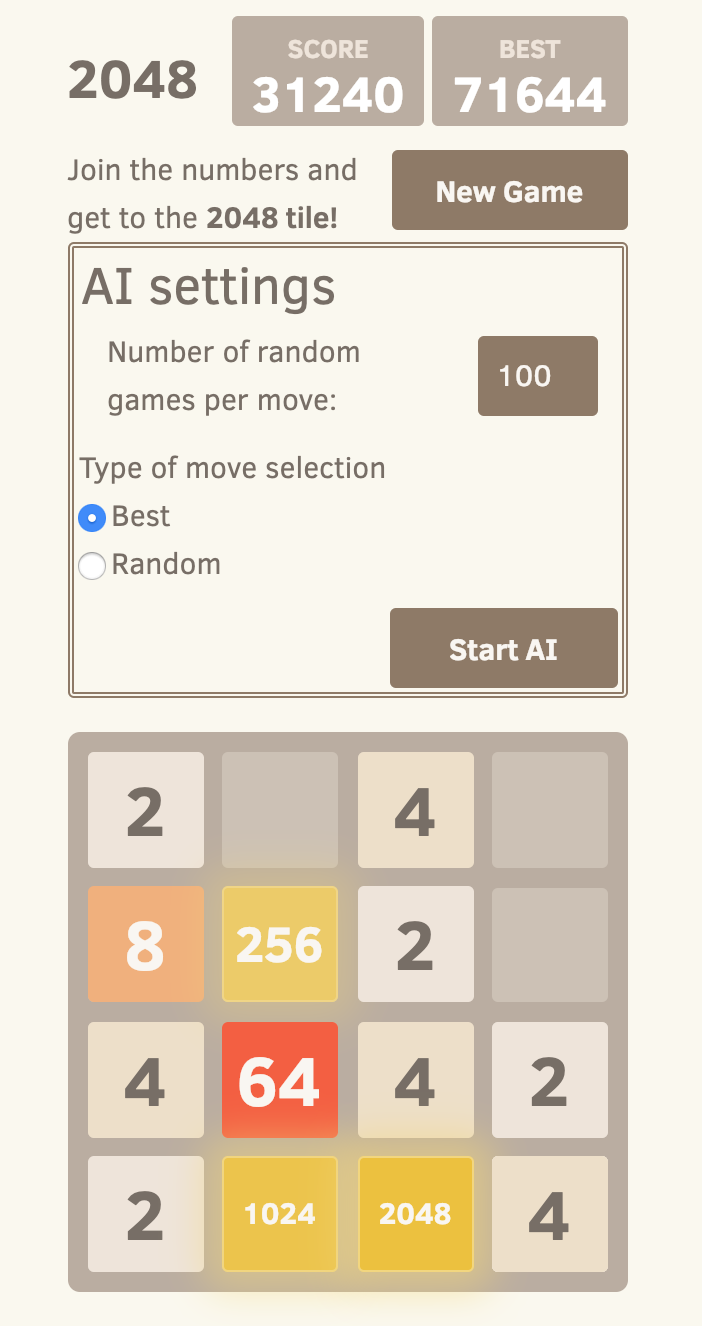
\includegraphics[scale=0.5]{igra.png}
\caption{Igra 2048 z uporabniškim vmesnikom za nastavljanje različnih konfiguracij umetne inteligence.}
\label{slika1}
\end{center}
\end{figure}

Rezultat se v igri računa tako, da se vsakič, ko igralec dve ploščici združi, rezultatu prišteje vrednost nove ploščice. Igra se najpogosteje igra na polju velikosti 4 x 4. Za polje take velikosti lahko naredimo največ ploščico z vrednostjo 131972, največji možen rezultat pa je 3,932,156. \ref{l1}

\section{Ideja}
V igri se ploščice na prazna polja postavljajo naključno, zato moramo uporabiti hevristični algoritem za iskanje naslednje poteze. Po raziskovanju po spletu \ref{l2} sem ugotovil, da večina ta problem reši tako, da poda programu omejitve kot naprimer, da se morajo ploščice z visokimi števili držati skupaj in ostati čim bolj v kotu, saj tako ostane več polj za druge ploščice. Ker sem želel, da program ne vsebuje znanja o igri in taktik, sem se namesto tega odločil za preprostejši pristop.

Glavna ideja algoritma, ki sem ga uporabil je, da če v vsako smer odigraš veliko število naključnih iger (prva poteza v željeno stran, vse naslednje pa naključno dokler se igra ne konča), se napake izenačijo in lahko ugotovimo, katera smer je za nas najbolj ugodna. Tako ob vsaki potezi algoritem odigra določeno število naključnih iger, izmed katerih vsaka vrne končni rezultat. Nato se iz teh rezultatov izracuna povprečje za vsako smer ter izbere poteza, pri kateri je povprečni rezultat najvišji.

Tak algoritem je požrešen, saj izbere potezo, ki mu v tem trenutku poda čim večji rezultat in se ne trudi ploščic razporejati v postavitev, ki mu bo kasneje dala večjo možnost, da pridobi boljši rezultat.

\section{Implementacija}
\subsection{Pripravljanje kode}
Z implementacijo sem začel tako, da sem iz github repozitorija na svoj računalnik naložil programsko kodo igre. Ta ni bila primerna za takojšnjo implementacijo umetne inteligence, saj se je grafični izris polja, ki ga igralec vidi, ob vsakem premiku spremenil. Tako sem del kode premaknil in malo spremenil tako, da se polje lahko spreminja neodvisno od grafičnega prikaza in kliče spremembo v grafičnem izrisu le po potrebi. Poleg tega sem v datoteko html dodal še del kode, ki uporabniku omogoča izbiro načina igre, število odigranih iger pri izbiri naslednje poteze ter gumb, s katerim umetno inteligenco igralec požene.

\subsection{Implementacija algoritma}
Ko je bila programska koda igre primerna za implementacijo algoritma, sem začel z kodo za iskanje najboljše poteze. To sem naredil tako, da sem napisal funkcijo, ki sprejme igralno polje ter vrne najboljšo potezo. V tej funkciji se za vsako od štirih strani odigra izbrano število igre tako, da je prva poteza v želeno smer, nato pa se poteze izbirajo naključno dokler se igra ne konča. Ko se taka (naključna) igra zaključi, vrne končni rezultat. Ti rezultati se nato seštejejo ter delijo s številom iger, da se dobi povprečen rezultat v vsako izmed smeri. Za tem se izbere poteza, ki ima najvišje povprečje. To potezo nato polje odigra ter osveži grafični prikaz.

Naredil sem tudi nekaj manjših optimizacij, da je algoritem hitreje ter bolje deloval. To sem naredil tako, da sem pred prvo potezo v določeno smer preveril, če se polje po njej spremeni. Če se polje spremeni je poteza veljavna, v nasprotnem primeru bo pa obstajala boljša poteza, zato sem rezultat za njo nastavil na nič. Poleg tega sem ugotovil, da je prvo potezo vsakič posebej potrebno izvesti, saj se v nasprotnem primeru naključna ploščica vedno pojavi na istem mestu, zaradi česar algoritem slabo oceni najboljšo potezo v primeru, da se nova ploščica pojavi na mestu različnem od tistega pri ocenjevanju. Grafični prikaz, ki ga uporabnik vidi, potrebuje nekaj časa da se osveži, zato je potrebno med vsakim klicem algoritma za iskanjem najboljše poteze počakati kratek čas. 

\subsection{Preizkušanje raznih taktik}
Pri Implementaciji sem poizkusil več različnih taktik za izračun uspešnosti posamezne naključne igre, a se je na koncu rezultat izkazal za najboljšega pokazatelja. Poleg tega sem poiskusil še število uspelih potez ter povprečno spremembo rezultata na potezo, a sta ti dobivali slabše rezultate kot le število točk (rezultat) po koncu naključne igre in ju zato nisem uporabljal.

\section{Rezultati}
\subsection{Moji rezultati}
Testiral sem več konfiguracij, ki sem jih ločil glede na število iger med potezami. Poleg tega sem preizkusil tudi igre z naključnimi potezami. Za vsako konfiguracijo sem odigral več iger ter dobil najnižji, najvišji ter povprečen rezultat čez vse igre, poleg tega pa procent iger, kjer je bila najvišja ploščica nad 2048 oziroma 4096. Rezultate sem prikazal v tabeli \ref{tab1}.

\begin{table}[htbp]
\caption{Število iger in uspeh}
\label{tab1}
\begin{center}
\begin{tabular}{llll}
\hline
število iger & najnižji/povprečni/najvišji rezultat & procent iger nad 2048/4096 & odigranih iger\\
\hline
naključna poteza & 232/1085.31/2760 & 0/0 & 100\\
1 & 488/4354.4/12048 & 0/0 & 150\\
10 & 1316/14746.96/35640 & 19/0 & 100\\
100 & 11632/38468.33/77700 & 91/24 & 100 \\
1000 & 71620 & 100/100 & 1 \\
\hline
\end{tabular}
\end{center}
\end{table}

Igro, ki je odigrala tisoč iger med vsako potezo sem pognal le enkrat, saj je igra predolgo trajala. Iz rezultatov je vidno, da več potez kot odigramo, boljši rezultat dobimo in da je že ena igra v vsako smer med potezami dovolj, da rezultat zelo povečamo glede na rezultat dobljen z naključnim izbiranjem potez. Opazi se lahko tudi, da se povprečni rezultat z vsakim dodatnim korakom poveča za veliko (relativno), ko je korakov malo, kasneje pa z dodatnim korakom ne pridobimo veliko več. Funkcija gledena število iger med koraki je naraščajoča in konveksna (podobna logaritmu).

\begin{figure}[h!]
\begin{center}
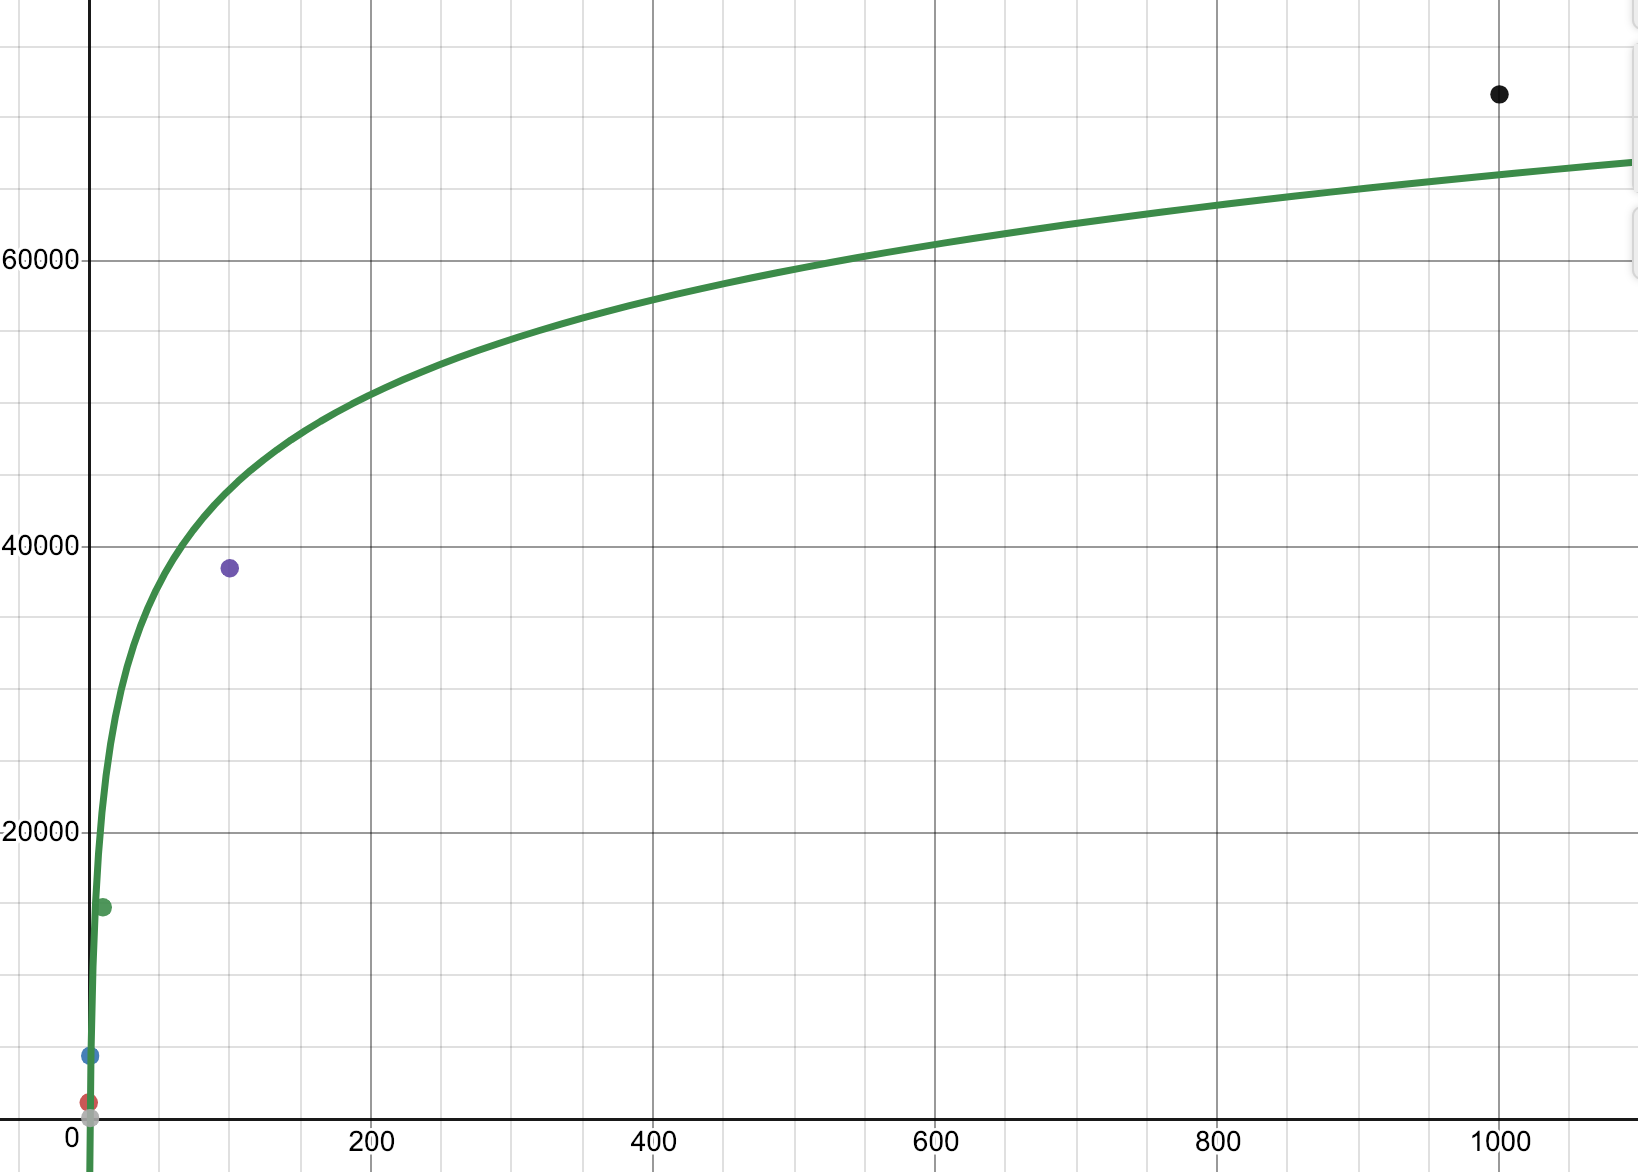
\includegraphics[scale=0.5]{aproxi.png}
\caption{Aproksimacija logaritma skozi dobljene točke.}
\label{slika2}
\end{center}
\end{figure}

\subsection{Primerjava z drugimi pristopi}
Po spletu sem poiskal še druge algoritme in jih primerjal z mojim. Algoritme je težko primerjati, saj je se na spletu najde veliko podobnih, ki pa dosegajo zelo različne rezultate. Tej algoritmi se razlikujejo v tem, da imajo večino že dodana neka pravila, ki jim olajšajo iskanje najboljše poteze ter pripomorejo k boljšemu rezultatu. Projekti ter algoritmi katere omenjam v nadaljevanju, so podrobneje navedeni na povezavah, ki se nahajajo med viri in literaturo.

\begin{description}
\item[pravilo urejenega igralnega polja]
Algoritem, ki uporablja pravilo, da mora biti največje ploščiče skupaj, urejene po vrsti in v enem od kotov nam da rezultat, ki je v povprečju boljši od mojega, a ta razlika ni zelo velika. Konkretna implementacija, ki sem jo našel je imela povprečen rezultat 42000. \ref{l3}

\item[nevronska mreža]
Pristop z nevronskimo mrežo pri tej igri ponavadi ni zelo uspešen, a sem našel projekt, v katerem je nevronska mreža prišla v povprečju do rezultata 85351. Tukaj je programer že podal v nevronsko mrežo nekaj pravil, navaja pa tudi nevronsko mrežo, ki ne pozna pravil, a vseeno zmaga igro z verjetnostjo 75 procentov. \ref{l4}

\item[minimax]
En izmed bolj uspešnih pristopov pri tej igri je minimax. Veliko projektov, ki uporablja ta algoritem pride brez problema do zmage. Projekt s tem pristopom, ki sem ga našel doseže zmago z verjetnostjo 71 procentov in povprečnim rezultatom 27250. To je manj od mojega pristopa, a ta pristop deluje hitreje. \ref{l5}

\item[expectimax]
Podobno kot minimax se tudi expectimax ponavadi zelo dobro obnese pri tej igri. Projekt z implementacijo minimax algoritma je imel poleg tudi implementacijo expectimax algoritma. Ta se je glede na povprečen rezultat bolje obnesel, saj je dobil v povprečju 29187 točk, a je zmago dosegel le v 64 procentih iger. \ref{l5}

\end{description}

\section{Zaključek}
Čeprav algoritem nima dodanih omejitev in je preprost, se ob sto igranih iger v vsako smer med potezami zelo dobro izkaže in igro zmaga v več kot devetdeset procentih iger. Če ta algoritem primerjamo z drugimi, ki uporabljajo omejitve, dobi slabše rezultate, a ti v večini primerov niso veliko boljši od tega pristopa. Algoritem bi se lahko izboljšalo tako, da bi se vanj dodalo razne omejitve oziroma nagrajevati boljše odločitve.

Pri izbiri sem si za cilj postavil zmagati to igro ter poizkusiti dobiti čim bojši rezultat. To mi je tudi uspelo, poleg tega sem pa ugotovil tudi, da je ta algoritem stabilen, saj pogosto pride do podobnega rezultata.

\setcounter{secnumdepth}{0}
\section{Viri in literatura}
\begin{enumerate}[label={[\arabic*]}]
  \item \label{l1} 2048 Wikipedia [Online]. Dosegljivo: \url{https://en.wikipedia.org/wiki/2048_(video_game)} (zadnji obisk 20.12.2018)
  \item \label{l2} Različni pristopi k reševanju igre 2048 [Online]. Dosegljivo: \url{https://stackoverflow.com/questions/22342854/what-is-the-optimal-algorithm-for-the-game-2048} (zadnji obisk 20.12.2018)
  \item \label{l3} Pristop urejenega igralnega polja [Online]. Dosegljivo: \url{https://nicola17.github.io/2014/03/26/an-artificial-intelligence-for-2048-game.html} (zadnji obisk 21.12.2018)
  \item \label{l4} Pristop z nevronsko mrežo [Online]. Dosegljivo: \url{https://github.com/tjwei/2048-NN} (zadnji obisk 21.12.2018)
  \item \label{l5} Minimax in expectimax pristop [Online]. Dosegljivo: \url{http://cs229.stanford.edu/proj2016/report/NieHouAn-AIPlays2048-report.pdf} (zadnji obisk 21.12.2018)
\end{enumerate}

\section{Izjava o izdelavi domače naloge.}
Domačo nalogo in pripadajoče programe sem izdelal sam.

\appendix
\appendixpage
Poleg poročila o seminarski nalogi prilagam še datoteko s programsko kodo. Ta je dostopna tudi na mojem \href{https://github.com/smeznar/2048}{Github repozitoriju}. Igro ter umetno inteligenco z različnimi konfiguracijami je pa možno tudi preizkusiti na \href{https://smeznar-ai-2048.herokuapp.com/#}{Spletni storitvi Heroku}. V njej so tudi vsi pridobljeni rezultati, ki sem jih dobil s testiranjem ter program s katerim sem izračunal rezultate, ki sem jih napisal v tabelo.
\end{document}
